\newpage

\section{Wyniki badań}

Pierwszy pomiar widma Ramana został zrobiony dla kryształka, który był na podłożu $\mathbf{GaP}$. Wzrost kryształków się odbywał na tym podłożu. 

\begin{figure}[H]
	\begin{center}
		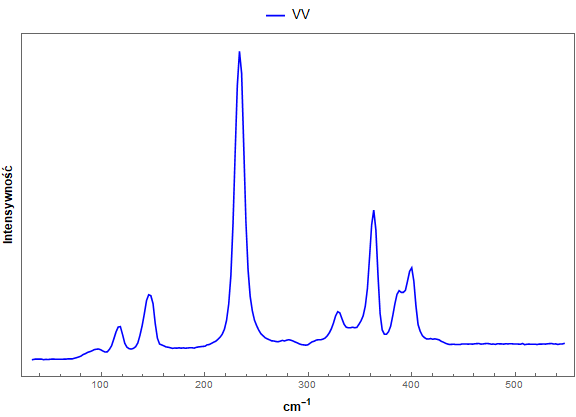
\includegraphics[width=0.8\linewidth]{Wyniki/Raman/plotGapWithGa2S3.png}
		\caption{Widmo Ramana dla $\mathbf{Ga_{2}S_{3}/GaP}$}
	\end{center}
\end{figure}

Piki 1,2,3,4,6 odpowiadają widmu Ramana dla $\mathbf{Ga_{2}S_{3}}$, a piki 5,7 odpowiadają widmu Ramana dla $\mathbf{GaP}$. Piki pochodzące z $\mathbf{GaP}$ znacznie utrudniają analizę piku 4 i 6. A poza tym można przypuszczać, że nie wszystkie piki, odpowiadające $\mathbf{Ga_{2}S_{3}}$ są widoczne z powodu obecności pików o numerach 5 i 7. 

Pomiary dla $\mathbf{Ga_{2}S_{3}/GaP}$ zostały zrobione tylko w konfiguracji VV, dlatego że później zostało postanowiono przenieść kryształki na inną powierzchnię aby pozbyć się niepożądanych pików na widmie Ramana. 

\newpage

Żeby to potwierdzić zostało uzyskane widmo Ramana dla $\mathbf{GaP}$, które pokazano na rysunku niżej:

\begin{figure}[H]
	\begin{center}
		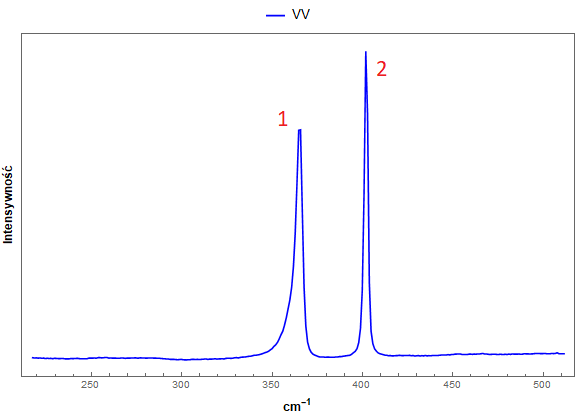
\includegraphics[width=0.8\linewidth]{Wyniki/Raman/plotGaP.png}
		\caption{Widmo Ramana dla $\mathbf{GaP}$. Piki 1 odpowiada przeunięciu około 360$cm^{-1}$, 2 -- 400$cm^{-1}$.}
	\end{center}
\end{figure}

\begin{figure}[H]
	\begin{minipage}[h]{0.5\linewidth}
		\center{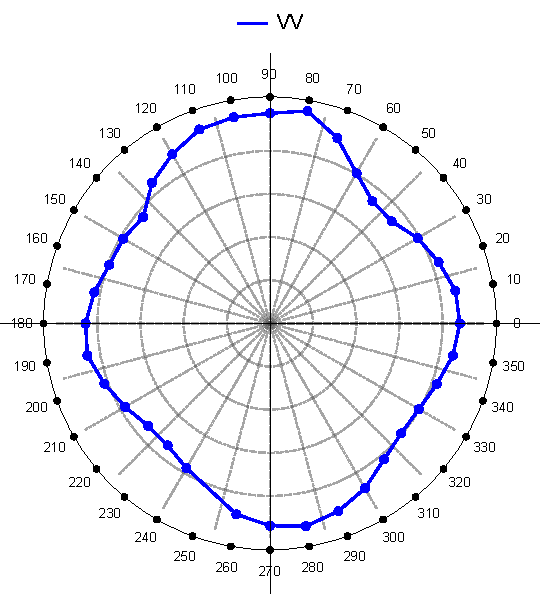
\includegraphics[width=0.8\linewidth]{Wyniki/WidmoPolaryzacyjne/plot5GaP.pdf}} \\ a) 
	\end{minipage}
	\hfill
	\begin{minipage}[h]{0.5\linewidth}
		\center{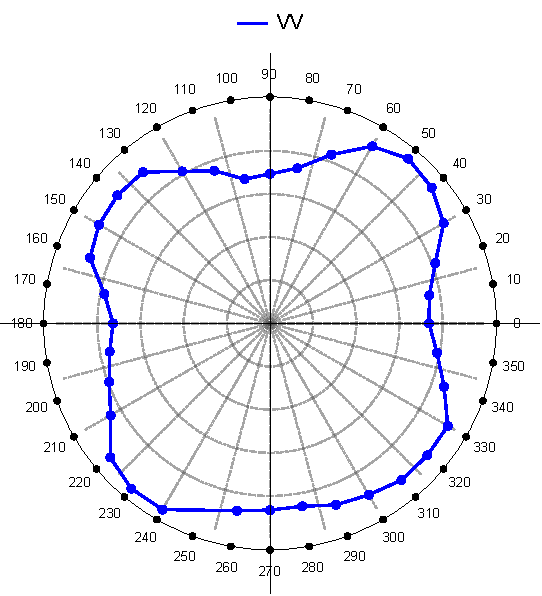
\includegraphics[width=0.8\linewidth]{Wyniki/WidmoPolaryzacyjne/plot7GaP.pdf}} \\b)
	\end{minipage}
	\caption{Widmo polaryzacyjne dla pików $\mathbf{GaP}$. a) Odpowiada piku 1, b) odpowiada piku 2.}
\end{figure}

Po zdrapani kryształków na szkło zostało uzyskane następujące widmo Ramana:

\begin{figure}[H]
	\begin{center}
		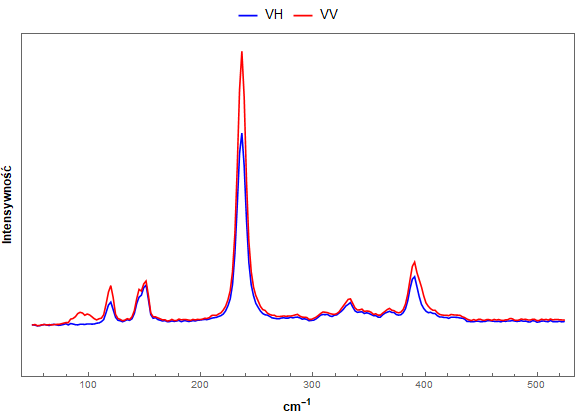
\includegraphics[width=0.8\linewidth]{Wyniki/Raman/plotVVandVH.png}
		\caption{Widmo Ramana dla $\mathbf{Ga_{2}S_{3}}$ bez wpływu $\mathbf{GaP}$ dla konfiguracji VV i VH.}
	\end{center}
\end{figure}

Na powyższym widmie Ramana zostały wyróżnione 7 pików. 1 $\rightarrow$ 117$cm^{-1}$, 2 $\rightarrow$ 143$cm^{-1}$, 3 $\rightarrow$ 149$cm^{-1}$, 4 $\rightarrow$ 235$cm^{-1}$, 5 $\rightarrow$ 309$cm^{-1}$, 6 $\rightarrow$ 330$cm^{-1}$, 7 $\rightarrow$ 390$cm^{-1}$. 

\begin{figure}[H]
	\begin{center}
		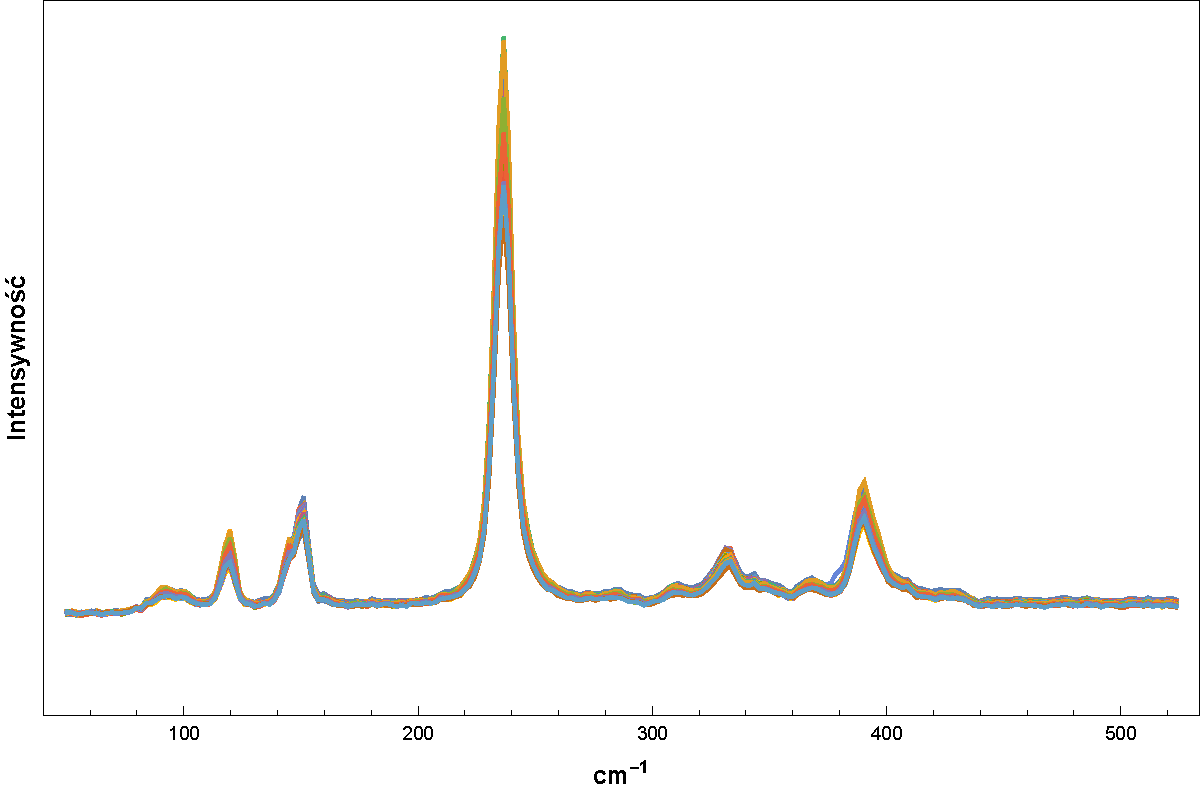
\includegraphics[width=0.8\linewidth]{Wyniki/Raman/plotAllVV.pdf}
		\caption{Widma ramanowskie dla 36 różnych kątów polaryzacji dla konfiguracji VV.}
	\end{center}
\end{figure}

\begin{figure}[H]
	\begin{center}
		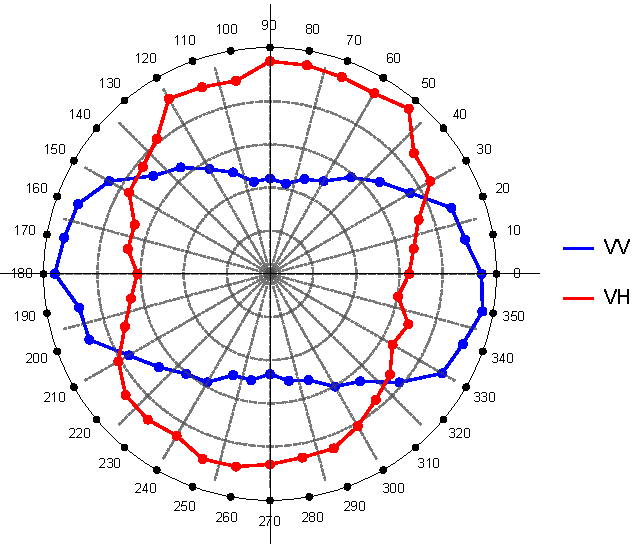
\includegraphics[width=0.75\linewidth]{Wyniki/WidmoPolaryzacyjne/plot117.pdf}
		\caption{Widmo polaryzacyjne dla pika 1 $\rightarrow$ 117$cm^{-1}$ }
	\end{center}
\end{figure}

\begin{figure}[H]
	\begin{center}
		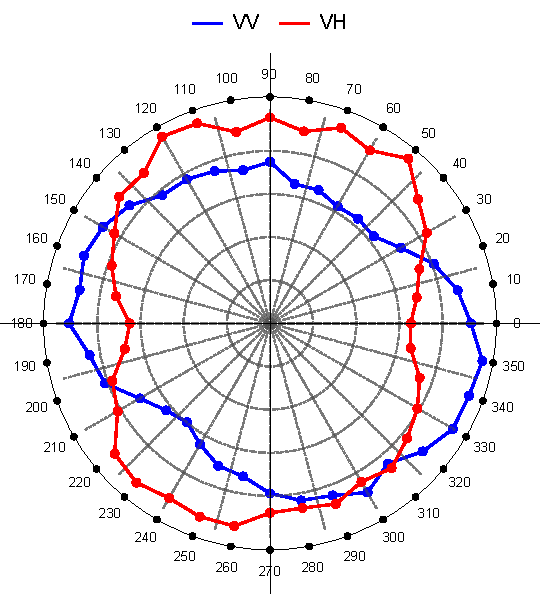
\includegraphics[width=0.75\linewidth]{Wyniki/WidmoPolaryzacyjne/plot143.pdf}
		\caption{Widmo polaryzacyjne dla pika 2 $\rightarrow$ 143$cm^{-1}$ }
	\end{center}
\end{figure}

\begin{figure}[H]
	\begin{center}
		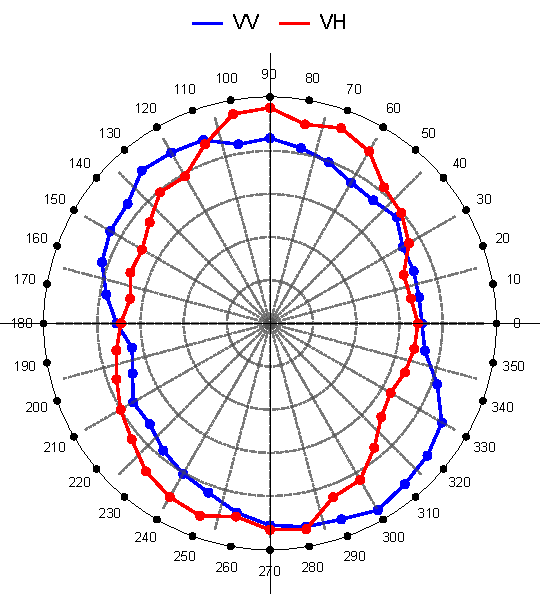
\includegraphics[width=0.75\linewidth]{Wyniki/WidmoPolaryzacyjne/plot149.pdf}
		\caption{Widmo polaryzacyjne dla pika 3 $\rightarrow$ 149$cm^{-1}$ }
	\end{center}
\end{figure}

\begin{figure}[H]
	\begin{center}
		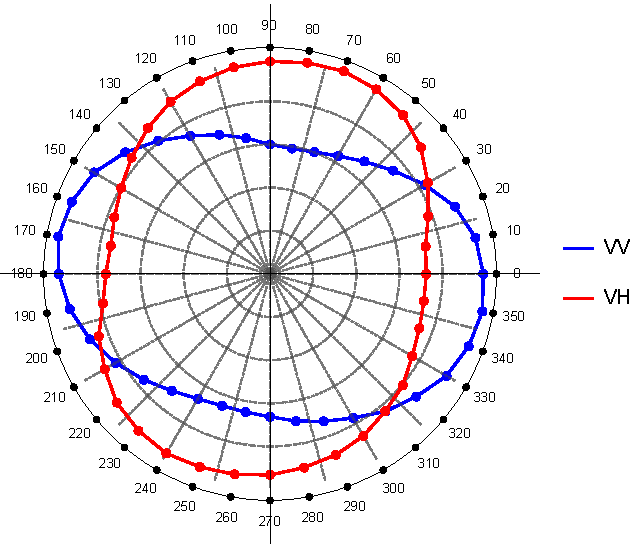
\includegraphics[width=0.75\linewidth]{Wyniki/WidmoPolaryzacyjne/plot235.pdf}
		\caption{Widmo polaryzacyjne dla pika 4 $\rightarrow$ 235$cm^{-1}$ }
	\end{center}
\end{figure}

\begin{figure}[H]
	\begin{center}
		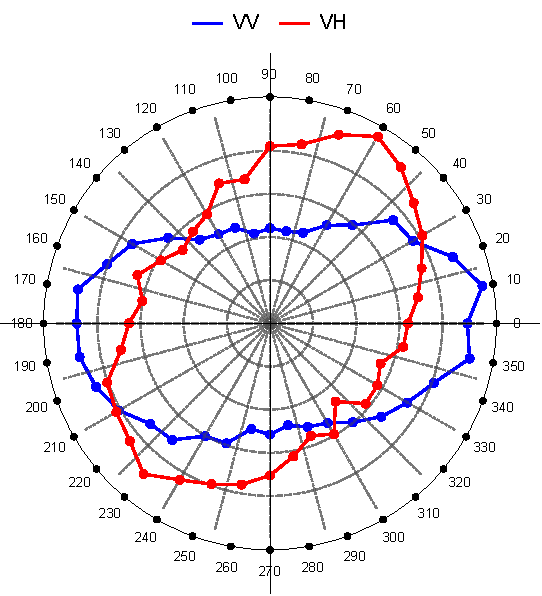
\includegraphics[width=0.75\linewidth]{Wyniki/WidmoPolaryzacyjne/plot309.pdf}
		\caption{Widmo polaryzacyjne dla pika 5 $\rightarrow$ 309$cm^{-1}$ }
	\end{center}
\end{figure}

\begin{figure}[H]
	\begin{center}
		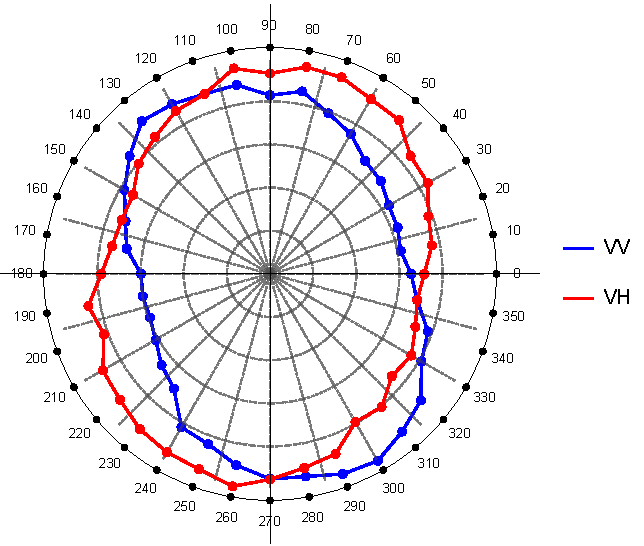
\includegraphics[width=0.75\linewidth]{Wyniki/WidmoPolaryzacyjne/plot330.pdf}
		\caption{Widmo polaryzacyjne dla pika 6 $\rightarrow$ 330$cm^{-1}$ }
	\end{center}
\end{figure}

\begin{figure}[H]
	\begin{center}
		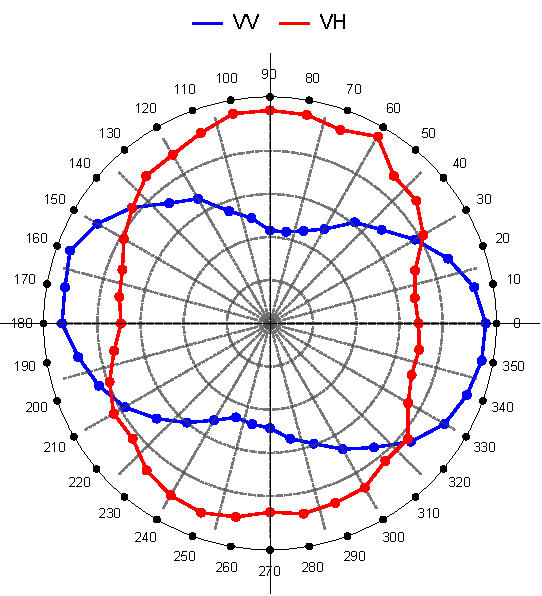
\includegraphics[width=0.75\linewidth]{Wyniki/WidmoPolaryzacyjne/plot390.pdf}
		\caption{Widmo polaryzacyjne dla pika 7 $\rightarrow$ 390$cm^{-1}$ }
	\end{center}
\end{figure}

\textbf{Zapytać.}


